% Clustering analysis
\subsection{Cluster analysis} \label{s:lit:clustering}

\subsubsection*{Models} \label{s:lit:cs_models}

Clustering algorithms have many variations, and these are covered in the code sample\footnote{See \href{https://scikit-learn.org/stable/modules/clustering.html}{blog post}.} from the Scikit-learn library \citep{Pedregosa2011-ts} from which a selection of methods are applied in this project; their applications on different datasets is displayed in \cref{fig:lit:clustering_types}. The rows represent different types of datasets and the columns are the algorithms covered in the project: K-means as a general-purpose algorithm, and both Ward and Agglomerative as hierarchical clustering methods, Gaussian Mixture Models and Spectral Clustering. It is worth mentioning that a modified version of the Scikit-learn code was adapted to meet the project's needs, enabling the running of multiple clustering techniques with varied parameters for TCGA dataset (see \cref{s:cs:right_config}) and networks' outputs (\cref{s:ap:p0_clustering,s:ap:N_II:clustering analysis}).

\paragraph*{K-means}

One of the most popular methods (and the simplest) is K-means clustering, which attempts to find patterns in the data by grouping data points their proximity. There are variations of the algorithm where datasets are split into multiple batches to improve performance (see \textit{MiniBatch K-means} from \cref{fig:lit:clustering_types}); or Fuzzy K-means \citep{Bezdek1984-ao} that output the cluster membership of each data point. This means that apart from the cluster labelling, there is additional information about how close each point is to a cluster\footnote{For example, if there are 3 clusters, a data point might be 90\% in cluster 1, 6\% in cluster 2, and 4\% in cluster 3.}. The pseudocode\footnote{Pseudocode is an accessible method to describe an algorithm.} for K-means is shown in \cref{code:k-means} and below are a few aspects of the model that are worth emphasising:
\begin{figure}[!t]
  \centering
  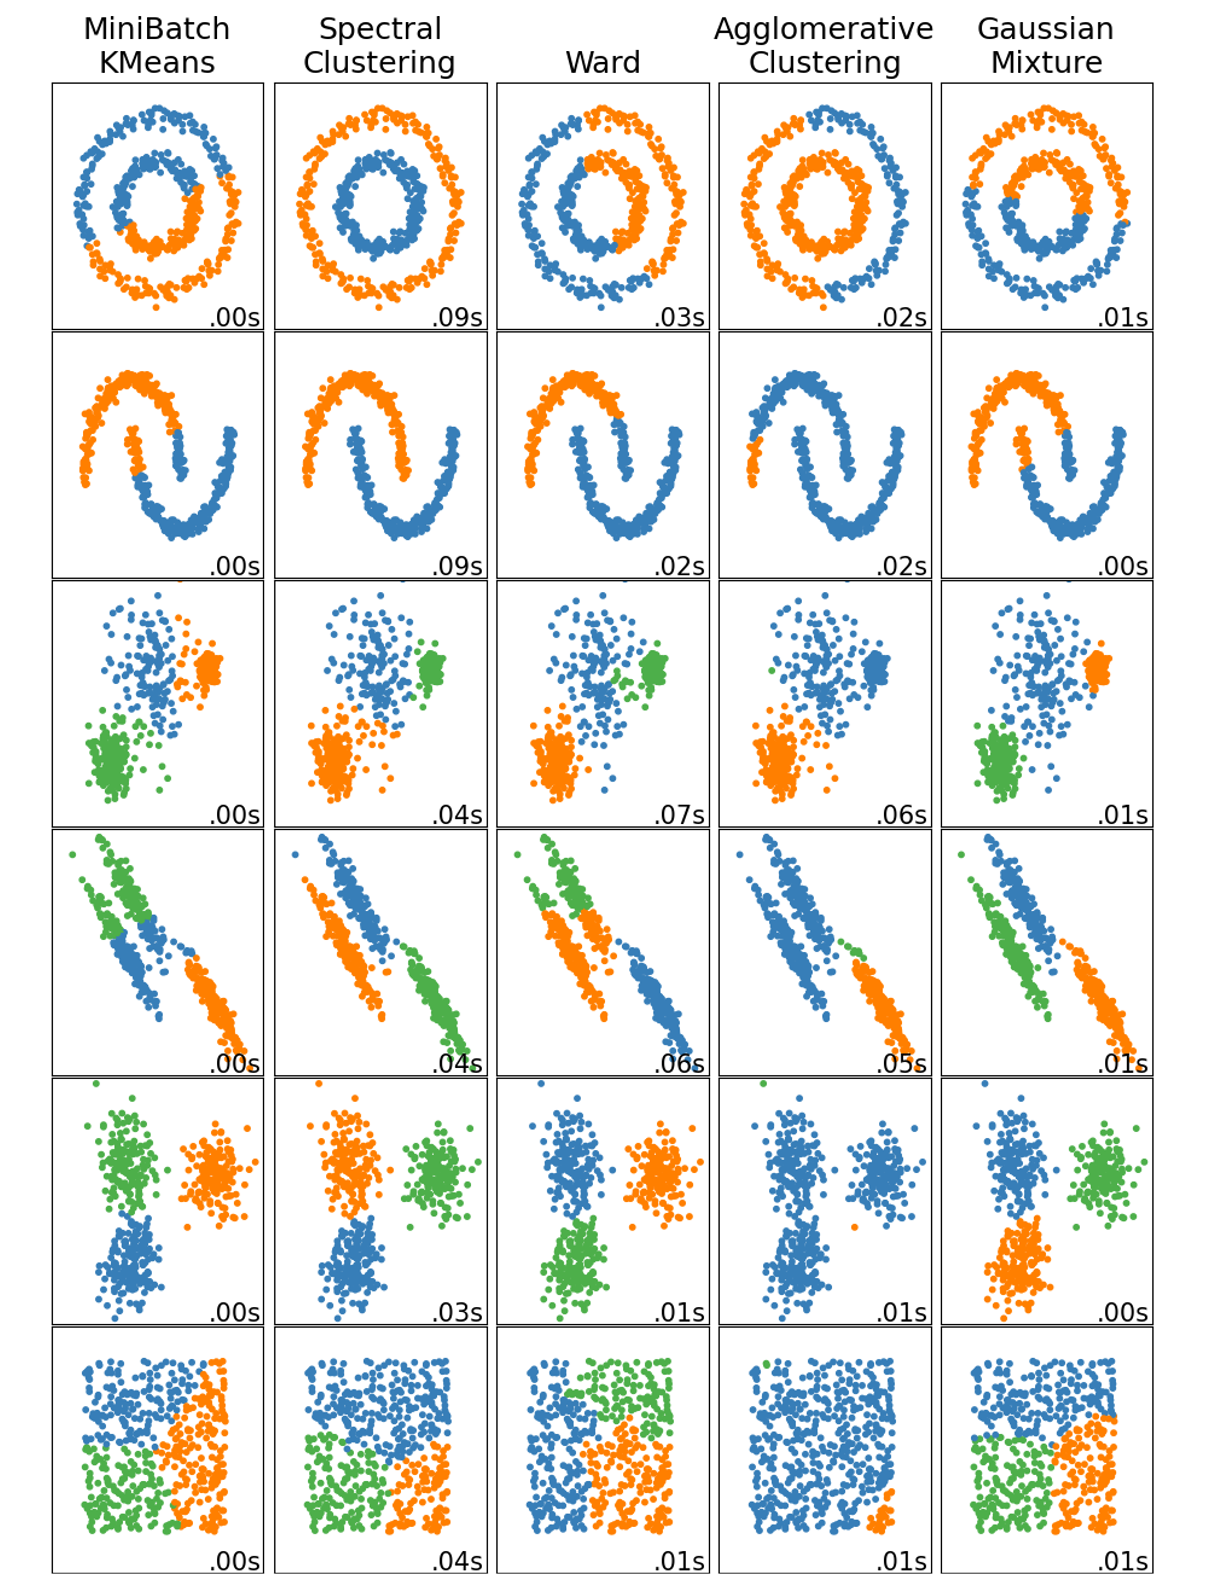
\includegraphics[width=0.8\textwidth,height=0.5\textheight,keepaspectratio]{Sections/Lit_review/Resources/clustering_scikit.png}
    \caption[Clustering models on different datasets]{How K-means (MiniBatch version), Spectral Clustering, Wards, Agglomerative Clustering, and Gaussian Mixture Models behave with different types of 2D datasets. Running times shown on the bottom right corner, all algorithms having comparable running times, with K-means being the fastest. Image adapted from \citet{Scikit-learn_undated-ax}.}
    \label{fig:lit:clustering_types}
\end{figure}

\begin{itemize}
  \item The number of centroids (K) is defined by the user.
  \item The distance between two points can be of different types; the Euclidean is the most common, but for higher dimensions, cosine is more suitable.
  \item Even though the centroids are randomly initialised, new values are computed at each step by averaging the distance of the points in that cluster to the old centroid.
  \item The algorithm converges when the centroids do not significantly change.
\end{itemize}

\begin{lstlisting}[float=!htb, caption={K-means pseudocode}, label={code:k-means}]
  1. Initialise k centroids at random positions
  2. while not converged do
     a. For each data point:
        i. Compute the distance to each centroid
        ii. Assign the data point to the cluster of the closest centroid
     b. For each cluster:
        i. Recalculate the centroid as the mean of all data points assigned to the cluster
     c. Check for convergence (e.g., centroids do not change or changes are below a threshold)
  3. end while
\end{lstlisting}


\paragraph*{Agglomerative clustering}

Agglomerative clustering is a type of hierarchical clustering that starts by considering each data point as its cluster and then computes higher up groups based on the given linkage method. These algorithms (pseudocode in \cref{code:agg_clustering}) build hierarchical trees and the output is visually represented by dendrogram figures, which are useful in visualising the clustering evolution. Both K-means and Agglomerative Clustering can use different types of distances, but the latter does not require specifying the number of groups. However, the dendrogram and the type of linkage method have to be set, configurations which influences algorithm, Scikit-learn supports the following parameters\footnote{There is a nice visualisation for each of these hierarchical clustering in this \href{https://towardsdatascience.com/machine-learning-algorithms-part-12-hierarchical-agglomerative-clustering-example-in-python-1e18e0075019}{Medium post}}:

\begin{itemize}
  \item \textbf{Average} - Grouping is done by the average distance between cluster points.
  \item \textbf{Ward} - Merging clusters by the sum of squared distances. This linkage minimises the variance and is similar to K-means.
  \item \textbf{Single} - The distance between two groups is given by the two closest points. This considers merging clusters that have the closest points.
  \item \textbf{Complete} - The opposite to Single linkage, the distance between the two groups is given by the farthest points. This method looks at the outer layer points and may provide a more accurate grouping.
\end{itemize}

The hierarchical clustering does not require the specification of the number of groups to be found in the dataset, but usually in practice the user needs to choose a dendrogram cut. This refers to how many groups are chosen from the hierarchical clustering, which is similar to the $K$ parameter in other algorithms for cluster size.


\begin{lstlisting}[float=!htb, caption={Agglomerative hierarchical clustering pseudocode}, label={code:agg_clustering}]
  1. Assign each data point to its own cluster
  2. while there is more than one cluster do
     a. Compute the distance between each pair of clusters
     b. Identify the two closest clusters
     c. Merge the two closest clusters into a single cluster
     d. Update the distance matrix to reflect the merge
  3. end while
  4. The final cluster can be represented as a dendrogram
\end{lstlisting}

\paragraph*{GMM and others}

Gaussian Mixture Models (GMM) are probabilistic models that assume all data points are generated from a mixture of a finite number of Gaussian distributions with unknown parameters. GMMs accommodate asymmetric clusters compared to K-means which assumes clusters are similar in size. Another applied clustering algorithm in the project, Spectral Clustering, transforms the clustering problem into a graph-partitioning problem. It begins by constructing an affinity matrix based on the pairwise similarity of points. It then uses linear algebra to project the data into a latent space from which the clusters are identified using methods such as K-means.

The clustering algorithms presented are used throughout the project, initially to establish a referential point independent of the methods used in other MIBC subtyping classifications \citep{Robertson2017-mg, Marzouka2018-ge, Kamoun2020-tj}. Then, the clustering models are used to stratify the output of the network approach.


% Clustering metrics
\subsubsection*{Cluster metrics} \label{s:lit:clustering_metrics}

One of the challenges in unsupervised learning is to measuring clustering performance as there is no labelling or prior information on the expected groups. This project uses the canonical metrics which are supported by Scikit-learn \citep{Pedregosa2011-ts,Scikit-learn_undated-ax}: Silhouette Coefficient, Calinski-Harabasz and Davies-Bouldin \citep{Rousseeuw1987-wy,Calinski1974-uu,Davies1979-tn}. 

All three scores are used across all the results chapters, in the clustering analysis (\cref{s:cs:right_config,fig:cs:sill_distrib}), first network approach developed in \cref{s:ap:p0_clustering} and the the more advanced network pipeline in \cref{s:ap:N_II:clustering analysis}.


\paragraph*{Silhouette Coefficient} \label{s:lit:silhouette}

The Silhouette Coefficient was introduced by \citet{Rousseeuw1987-wy} with the goal of finding the appropriate clustering configuration. The score takes into account both how close and how separated the groups are, and it does not require knowing the number of clusters in advance. For each point (or sample), a silhouette value is calculated using \cref{eq:cs:sil}, where \(a\) is the average distance from the sample to all other points within its cluster, while \(b\) is the average distance from the sample to points in the nearest other cluster. Thus, \(a\) measures the cohesion (how close the points in the cluster are), and \(b\) measures the separation from other clusters. The cosine distance is used throughout this project to compute the distances for the Silhouette scores.

\begin{equation} \label{eq:cs:sil}
    s = \frac{b - a}{\max(a, b)}
\end{equation}

In the work that introduced the Silhouette score \citep{Rousseeuw1987-wy}, the author indicates that positive values (closer to 1) indicate well-separated groups, while negative values denote mis-clustering of the samples, and scores around 0 suggest that a sample could belong to multiple clusters. As a midpoint between 0 and 1, Silhouette values \(>\)0.5 are considered to indicate well-clustered data points.


\paragraph*{Calinski-Harabasz} \label{s:lit:cal_harab}


The Calinski-Harabasz Index was introduced by \citet{Calinski1974-uu} with the same goal as the Silhouette score: to help find the number of clusters that yields the best group separation and the most densely connected clusters. The metric is computed by \cref{eq:cs:cal_harab}, where \(\mathrm{tr}(B_k)\) is the trace of the between-cluster dispersion matrix. The matrix \(B_k\) represents the dispersion between the centroids (i.e., the centres of each cluster) and the overall mean of the data, while the trace is the sum of the diagonal elements of this matrix; the larger the trace, the better separated the groups are. The \(\mathrm{tr}(W_k)\) is the trace of the within-cluster dispersion matrix \(W_k\), which measures the dispersion of data points within each cluster, where smaller values indicate that the points within the groups are closer together. The \(n_E\) represents the total number of data points, while \(k\) is the number of clusters.

\begin{equation} \label{eq:cs:cal_harab}
    s = \frac{\mathrm{tr}(B_k)}{\mathrm{tr}(W_k)} \times \frac{n_E - k}{k - 1}
\end{equation}

In short, the first term in \cref{eq:cs:cal_harab} is the ratio between the dispersion of the cluster centroids (indicating how well-separated the clusters are) and the dispersion within clusters (indicating how tightly the data points within each cluster are grouped); higher values mean better-defined groups. The second part of the equation accounts for the number of data points and the number of clusters. Overall, higher values of the Calinski-Harabasz Index indicate that the clusters are better defined.


\paragraph*{Davies-Bouldin} \label{s:lit:davies_bouldin}

The third metric used to determine the cluster configuration is the Davies-Bouldin Index, introduced by \citet{Davies1979-tn}, which measures the separation and compactness of clusters. The metric is computed by the first equation in \cref{eq:cs:davies_bouldin}, where \(k\) is the number of clusters, and \(i, j\) denote the cluster indices. \(R_{ij}\) is the similarity measure defined by \cref{eq:cs:davies_bouldin_similarity}, where \(s_i\) is the average distance of the points in cluster \(i\) to the centroid of that cluster, while \(d_{ij}\) is the distance between the centroids of clusters \(i\) and \(j\).

\begin{equation} \label{eq:cs:davies_bouldin}
    DB = \frac{1}{k} \sum_{i=1}^k \max_{i \neq j} R_{ij}
\end{equation}

\begin{equation} \label{eq:cs:davies_bouldin_similarity}
    R_{ij} = \frac{s_i + s_j}{d_{ij}}
\end{equation}

As in the case of the other two metrics, the Davies-Bouldin Index takes into account both the dispersion within clusters and the separation between clusters. However, lower values are better for this metric, as it indicates better cluster separation and compactness, i.e., larger values of \(d_{ij}\) and smaller values of \(s_i\) and \(s_j\).


% Dimension reduction
\subsection{Dimension reduction} \label{s:lit:dim_red}

In contrast to many computationally or physics-focused data analysis problems, biologically derived datasets are characterised by a high number of features (dimensions) and a small number of samples, making it necessary to use dimensionality reduction. Furthermore, most features are not truly independent; instead, they represent multiple measures of different components of linked and often self-regulating molecular pathways. To address the imbalance between the number of samples and features, dimension reduction techniques compress the information into more manageable parts. One of the most popular is \acrfull{pca} \citep{Hotelling1936-qq, Pearson1901-zd}, which projects the higher-dimensional data onto a specified lower-dimensional space. The method uses linear algebra techniques such as Singular Value Decomposition (SVD) to compress the variance into a reduced set of dimensions.

% I think you should spin PCA as being useful for many bio questions because of such high co-correlation and co-dependency of measured features, rather than seeing that as a weakness. Your limitations bit stands, but dimension reduction remains very important for bio data

% Variance and its importance
Variance is important as it explains how much the data points differ from each other, which can also be thought of as a proxy for the 'interesting' aspects of the data. For example, when the samples in a dataset do not vary a lot, it is easier to describe the information present; in this case, fewer principal components (PCs) are needed. Conversely, when the data points have a high variance, the dataset is more complex, and more PCs are required to adequately represent the dataset.

% Where PCA is useful
In simple cases, the variance between biological sexes across the dataset's samples can be represented by a single PC instead of the expression of a few specific genes. In more complex situations, such as in this project, the PCs may encode genetic variation that is specific to a subtype. For example, the first two components often encode for the Basal and Luminal phenotypes of MIBC, as seen in the cluster plot from the cluster analysis pipeline \cref{fig:cs:clustering_pipeline}.

PCA is extensively used in this project, initially to reduce the dimensionality of the data, and subsequently as a proxy metric to gauge the amount of variance contained in a subset of genes. The work in \cref{s:clustering_analysis} covers the cluster analysis used in the project, where the methods for determining the number of PCs are discussed in \cref{s:cs:right_config}, along with the effects of dimensionality reduction on the clustering metrics.


\subsubsection*{Limitations}

While \acrshort{pca} is the main dimensionality reduction method used in this project, it has certain limitations, primarily its poor performance on non-linear datasets. To address these shortcomings, \acrfull{umap} and \acrfull{tsne} were developed by \citep{McInnes2018-dz,Hinton2002-pz} . Both are stochastic and non-linear dimensionality reduction techniques widely used in bioinformatics. UMAP has been gaining popularity as it is more stable in representing both within- and between-cluster sample relatedness. However, while UMAP is effective at reducing data dimensionality, its visualisations can be misleading, as the proximity of points and clusters does not necessarily represent the 'closeness' of the data \citep{Chari2023-et}. When applying these techniques, it is advisable to perform clustering first and then use UMAP/t-SNE for visualisation.

Another dimensionality reduction technique is \acrfull{nmf} \citep{Lee1999-fj}, which operates on similar principles to PCA by finding a matrix of lower rank with minimal information loss. This approach means that features important to the data are better preserved when reduced to lower dimensions, while those that do not contribute significantly to data resolution are discarded. Additionally, NMF conserves the non-linear aspects of the data, and a Bayesian version of it has been used in \acrlong{tcga} classification \citep{Robertson2017-mg}. NMF is also used in the work of propagating mutation data into networks by \citet{Yang2016-dm, Cai2008-fv}, and this is further discussed in \cref{s:lit:net_prop}.

